\chapter{Additive White Gaussian Noise (AWGN)}
\label{ch:awgn}

\begin{nontechnical}
\textbf{AWGN is the ``static'' or ``hiss'' you hear on old radios}---random interference that corrupts signals no matter how strong they are.

\textbf{Simple idea:}
\begin{itemize}
\item Every electronic system generates random noise from heat
\item This noise follows a bell-curve (Gaussian) pattern
\item It adds to your signal, making it harder to decode correctly
\end{itemize}

\textbf{Real-world examples:}
\begin{itemize}
\item \textbf{Old TV static}: Random snow when you lose the signal
\item \textbf{Grainy photos in low light}: Camera sensors produce AWGN when there's not enough light
\item \textbf{FM radio hiss}: Background noise when tuned between stations
\item \textbf{Bluetooth stuttering}: Weak signals get corrupted by thermal noise
\end{itemize}

\textbf{Why it matters:} AWGN represents the \textbf{fundamental physical limit} on communication. You can't eliminate it (it comes from quantum thermal motion), but you can overcome it with more power, error correction, or better antennas. Every communication system is designed around beating AWGN.
\end{nontechnical}

\section{Overview}

\textbf{Additive White Gaussian Noise (AWGN)} is the most fundamental noise model in communication theory, representing the random thermal noise present in all electronic systems.

\begin{keyconcept}
The AWGN model is the \textbf{gold standard} for analyzing communication system performance. It provides a tractable mathematical framework while representing the dominant noise source in most practical systems: thermal noise from electronic components.
\end{keyconcept}

The acronym AWGN describes three critical properties:

\begin{itemize}
\item \textbf{Additive}: Noise combines with the signal linearly: $r(t) = s(t) + n(t)$
\item \textbf{White}: Power spectral density is constant across all frequencies (like white light)
\item \textbf{Gaussian}: Amplitude distribution follows the normal (Gaussian) probability distribution
\end{itemize}

AWGN serves as the baseline for all modulation scheme comparisons and is the foundation for calculating theoretical bit error rates (BER) and channel capacity.

\section{Mathematical Description}

\subsection{Time-Domain Model}

The received signal in an AWGN channel is expressed as:
\begin{equation}
r(t) = s(t) + n(t)
\end{equation}
where:
\begin{itemize}
\item $r(t)$ = received signal (volts)
\item $s(t)$ = transmitted signal (volts)
\item $n(t)$ = additive white Gaussian noise (volts)
\end{itemize}

\subsection{Statistical Properties}

The noise process $n(t)$ is characterized by:

\textbf{1. Zero mean:}
\begin{equation}
E[n(t)] = 0
\end{equation}

\textbf{2. Variance (noise power):}
\begin{equation}
\sigma^2 = E[n^2(t)] = N_0/2
\end{equation}
where:
\begin{itemize}
\item $\sigma^2$ = noise variance (watts)
\item $N_0$ = noise power spectral density (W/Hz)
\end{itemize}

\textbf{3. Probability density function:}
\begin{equation}
p(n) = \frac{1}{\sqrt{2\pi\sigma^2}} e^{-\frac{n^2}{2\sigma^2}}
\end{equation}

This is the famous bell curve, centered at zero with standard deviation $\sigma$.

\subsection{Gaussian Distribution Visualization}

The probability density function shows the classic bell curve shape:

\begin{center}
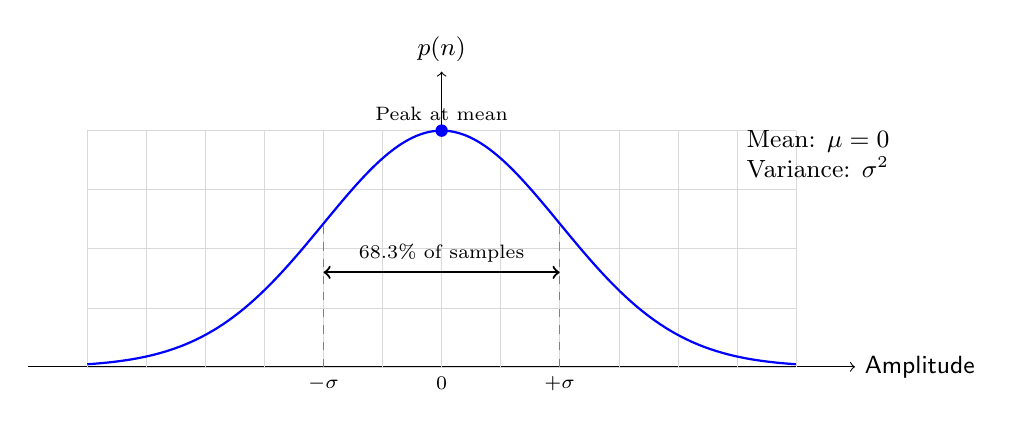
\begin{tikzpicture}[scale=1.5]
% Axes
\draw[->] (-3.5,0) -- (3.5,0) node[right] {\sffamily\small Amplitude};
\draw[->] (0,0) -- (0,2.5) node[above] {\sffamily\small $p(n)$};

% Grid
\draw[very thin,gray!30] (-3,0) grid[step=0.5] (3,2);

% Gaussian curve (approximated with plot)
\draw[thick,blue] plot[smooth,domain=-3:3,samples=100] 
  (\x, {2*exp(-\x*\x/2)});

% Standard deviation markers
\draw[dashed,gray] (-1,0) -- (-1,1.2);
\draw[dashed,gray] (1,0) -- (1,1.2);
\node[below,font=\scriptsize] at (-1,0) {$-\sigma$};
\node[below,font=\scriptsize] at (1,0) {$+\sigma$};
\node[below,font=\scriptsize] at (0,0) {$0$};

% Annotations
\draw[<->,thick] (-1,0.8) -- (1,0.8) node[midway,above,font=\scriptsize] {68.3\% of samples};
\node[right,font=\small,align=left] at (2.5,1.8) {Mean: $\mu = 0$\\Variance: $\sigma^2$};

% Peak label
\fill[blue] (0,2) circle (1.5pt);
\node[above,font=\scriptsize] at (0,2) {Peak at mean};
\end{tikzpicture}
\end{center}

\textbf{Key observation:} 68.3\% of noise samples fall within $\pm\sigma$, 95.4\% within $\pm2\sigma$, and 99.7\% within $\pm3\sigma$.

\section{AWGN Channel Model}

\subsection{Block Diagram Representation}

The AWGN channel is the simplest channel model in communications:

\begin{center}
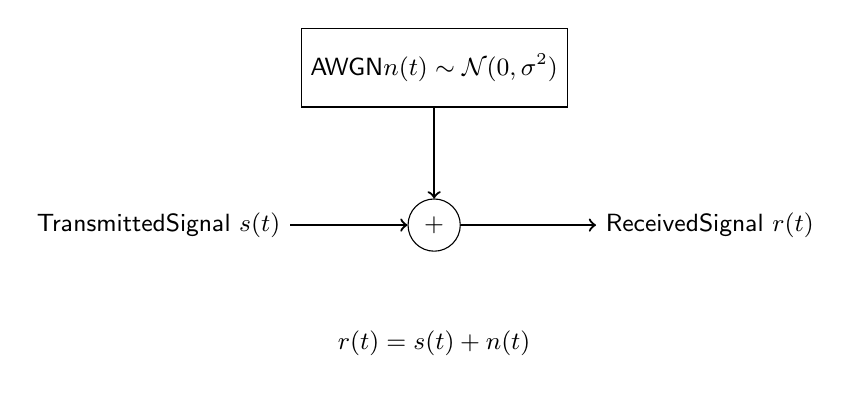
\begin{tikzpicture}[
  block/.style={rectangle, draw, minimum width=2.5cm, minimum height=1cm, font=\sffamily\small},
  node distance=3cm,
  font=\small
]
\node (input) {\sffamily Transmitted\\Signal $s(t)$};
\node[circle, draw, right of=input, node distance=3.5cm] (sum) {$+$};
\node[right of=sum, node distance=3.5cm] (output) {\sffamily Received\\Signal $r(t)$};
\node[block, above of=sum, node distance=2cm] (noise) {AWGN\\$n(t) \sim \mathcal{N}(0, \sigma^2)$};

% Arrows
\draw[->,thick] (input) -- (sum);
\draw[->,thick] (noise) -- (sum);
\draw[->,thick] (sum) -- (output);

% Equation annotation
\node[below of=sum, node distance=1.5cm, font=\small] {$r(t) = s(t) + n(t)$};
\end{tikzpicture}
\end{center}

\subsection{Complex Baseband (I/Q) Representation}

In the I/Q plane, AWGN adds independent Gaussian noise to both components:

\textbf{Received symbol:}
\begin{equation}
r = s + n = (I_s + jQ_s) + (n_I + jn_Q)
\end{equation}
where:
\begin{itemize}
\item $s = I_s + jQ_s$ = transmitted complex symbol
\item $n = n_I + jn_Q$ = complex noise
\item $n_I, n_Q \sim \mathcal{N}(0, \sigma^2)$ are independent
\end{itemize}

\textbf{Component equations:}
\begin{equation}
I_r = I_s + n_I
\end{equation}
\begin{equation}
Q_r = Q_s + n_Q
\end{equation}

The independence of $n_I$ and $n_Q$ is crucial---noise corrupts both dimensions equally and uncorrelated.

\subsection{Impact on Constellation Diagrams}

AWGN causes transmitted constellation points to spread into clouds. The higher the noise power, the larger the cloud:

\begin{center}
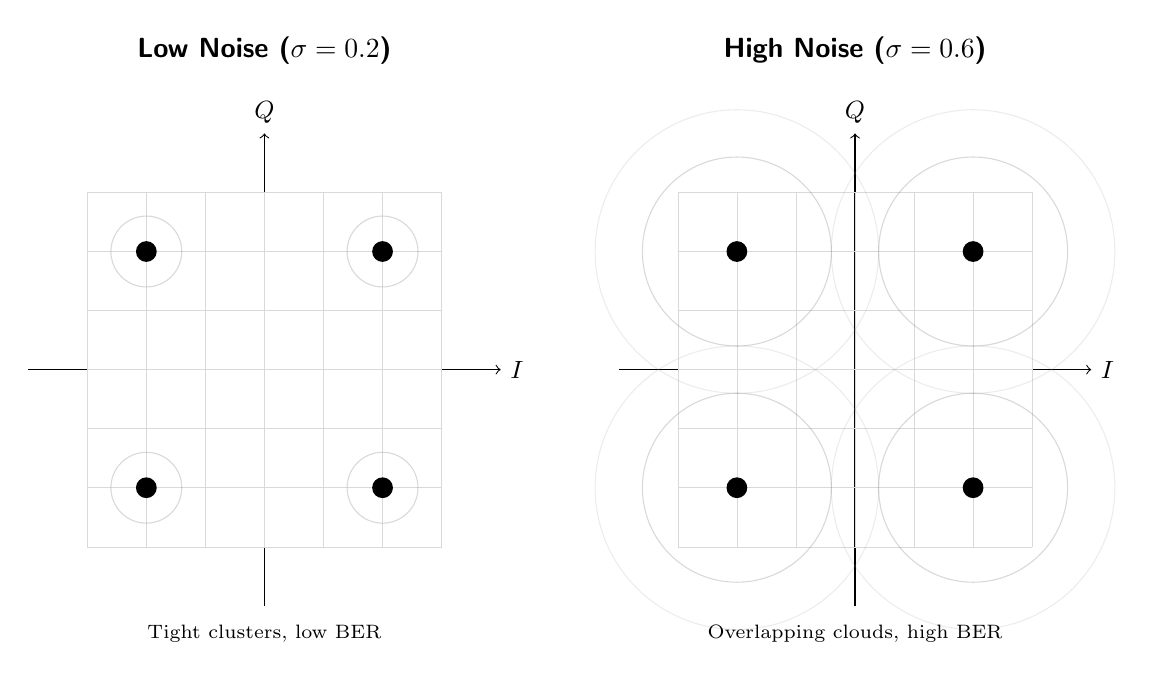
\begin{tikzpicture}[scale=1.5]
% Low noise constellation (left)
\begin{scope}[shift={(0,0)}]
\node[above,font=\sffamily\bfseries] at (0,2.5) {Low Noise ($\sigma = 0.2$)};
\draw[->] (-2,0) -- (2,0) node[right,font=\sffamily\small] {$I$};
\draw[->] (0,-2) -- (0,2) node[above,font=\sffamily\small] {$Q$};
\draw[very thin,gray!30] (-1.5,-1.5) grid[step=0.5] (1.5,1.5);

% QPSK constellation with small noise
\fill[black] (1,1) circle (2.5pt);
\fill[black] (-1,1) circle (2.5pt);
\fill[black] (-1,-1) circle (2.5pt);
\fill[black] (1,-1) circle (2.5pt);

% Noise clouds (small)
\foreach \x/\y in {1/1, -1/1, -1/-1, 1/-1} {
  \draw[gray,opacity=0.3] (\x,\y) circle (0.3);
}

\node[below=12pt,font=\scriptsize] at (0,-1.8) {Tight clusters, low BER};
\end{scope}

% High noise constellation (right)
\begin{scope}[shift={(5,0)}]
\node[above,font=\sffamily\bfseries] at (0,2.5) {High Noise ($\sigma = 0.6$)};
\draw[->] (-2,0) -- (2,0) node[right,font=\sffamily\small] {$I$};
\draw[->] (0,-2) -- (0,2) node[above,font=\sffamily\small] {$Q$};
\draw[very thin,gray!30] (-1.5,-1.5) grid[step=0.5] (1.5,1.5);

% QPSK constellation with large noise
\fill[black] (1,1) circle (2.5pt);
\fill[black] (-1,1) circle (2.5pt);
\fill[black] (-1,-1) circle (2.5pt);
\fill[black] (1,-1) circle (2.5pt);

% Noise clouds (large, overlapping)
\foreach \x/\y in {1/1, -1/1, -1/-1, 1/-1} {
  \draw[gray,opacity=0.3] (\x,\y) circle (0.8);
  \draw[gray,opacity=0.15] (\x,\y) circle (1.2);
}

\node[below=12pt,font=\scriptsize] at (0,-1.8) {Overlapping clouds, high BER};
\end{scope}
\end{tikzpicture}
\end{center}

\textbf{Key insight:} When noise clouds overlap, the receiver can't reliably distinguish between symbols, causing bit errors.

\section{Noise Power and SNR Relationships}

\subsection{Signal-to-Noise Ratio}

The fundamental performance metric is the signal-to-noise ratio (SNR):
\begin{equation}
\mathrm{SNR} = \frac{P_s}{P_n} = \frac{E[s^2(t)]}{E[n^2(t)]} = \frac{P_s}{\sigma^2}
\end{equation}
where:
\begin{itemize}
\item $P_s$ = signal power (watts)
\item $P_n = \sigma^2$ = noise power (watts)
\end{itemize}

In decibels:
\begin{equation}
\mathrm{SNR}_{\mathrm{dB}} = 10\log_{10}\left(\frac{P_s}{\sigma^2}\right)
\end{equation}

\subsection{Energy per Bit to Noise Ratio}

For digital communications, the more fundamental metric is $E_b/N_0$:
\begin{equation}
\frac{E_b}{N_0} = \frac{E_b}{\sigma^2} = \frac{P_s T_b}{\sigma^2}
\end{equation}
where:
\begin{itemize}
\item $E_b$ = energy per bit (joules)
\item $T_b$ = bit duration (seconds)
\item $N_0 = 2\sigma^2$ = noise power spectral density (W/Hz)
\end{itemize}

\textbf{Relationship to SNR:}
\begin{equation}
\frac{E_b}{N_0} = \frac{\mathrm{SNR} \cdot B}{R_b}
\end{equation}
where $B$ is bandwidth (Hz) and $R_b$ is bit rate (bps).

\section{Physical Origins of AWGN}

\subsection{Thermal Noise}

The dominant source of AWGN in most systems is \textbf{thermal noise} (Johnson-Nyquist noise):

\begin{equation}
P_n = kTB
\end{equation}
where:

\begin{itemize}
\item $k = 1.38 \times 10^{-23}$ J/K = Boltzmann's constant
\item $T$ = absolute temperature (Kelvin)
\item $B$ = bandwidth (Hz)
\end{itemize}

\begin{calloutbox}{Example: Thermal Noise at Room Temperature}
At $T = 290$ K (room temperature) over $B = 1$ MHz:
\begin{equation}
P_n = (1.38 \times 10^{-23})(290)(10^6) = 4.0 \times 10^{-15}\ \text{W} = -114\ \text{dBm}
\end{equation}
This is the fundamental noise floor that cannot be eliminated.
\end{calloutbox}

\subsection{Other Noise Sources}

While thermal noise dominates, other sources contribute:

\begin{itemize}
\item \textbf{Shot noise}: Discrete nature of charge carriers (important in photodetectors)
\item \textbf{Flicker noise (1/f noise)}: Low-frequency noise in semiconductors
\item \textbf{Amplifier noise}: Additional noise from active components (characterized by noise figure)
\item \textbf{Cosmic

 noise}: Cosmic microwave background (2.7 K, negligible at most frequencies)
\item \textbf{Interference}: When many independent interferers combine, Central Limit Theorem makes total interference approximately Gaussian
\end{itemize}

\begin{keyconcept}
The \textbf{Central Limit Theorem} explains why Gaussian noise is so common: when many independent random noise sources add together, their sum tends toward a Gaussian distribution, regardless of individual source distributions.
\end{keyconcept}

\section{Why AWGN is the Standard Model}

\subsection{Theoretical Justifications}

\begin{enumerate}
\item \textbf{Mathematical tractability}: Gaussian statistics enable closed-form BER expressions
\item \textbf{Fundamental limit}: Thermal noise is unavoidable---it's the quantum floor
\item \textbf{Realistic approximation}: Many real channels (satellite, line-of-sight radio) are AWGN-dominated
\item \textbf{Worst-case Gaussian}: Among all distributions with given variance, Gaussian maximizes entropy (most uncertainty)
\item \textbf{Benchmark standard}: Industry uses AWGN as baseline for all comparisons
\end{enumerate}

\subsection{When AWGN Model is Appropriate}

\textbf{Good approximation:}
\begin{itemize}
\item Deep-space communications (Voyager, Mars missions)
\item Satellite downlinks (clear weather)
\item Cable systems (coaxial, fiber with optical amplifiers)
\item Line-of-sight microwave links
\item High SNR systems where noise dominates over fading
\end{itemize}

\textbf{Poor approximation:}
\begin{itemize}
\item Mobile cellular (multipath fading dominates)
\item Indoor WiFi (Rayleigh/Rician fading)
\item Underwater acoustic (impulsive noise)
\item Power-line communications (impulsive interference)
\end{itemize}

\begin{warningbox}
AWGN analysis provides \textbf{optimistic} BER estimates for fading channels. Real mobile systems experience 10-20 dB worse performance than AWGN predictions unless diversity or coding is employed.
\end{warningbox}

\section{Worked Example: Link Budget with AWGN}

\textbf{Problem:} A satellite ground station receives a BPSK signal. Calculate the achieved bit error rate.

\subsection*{Given Parameters}

\begin{tabular}{@{}ll@{}}
Received signal power & $P_s = -100$ dBm \\
System temperature & $T_s = 200$ K \\
Bandwidth & $B = 1$ MHz \\
Bit rate & $R_b = 500$ kbps \\
Modulation & BPSK (coherent) \\
\end{tabular}

\subsection*{Required}
Find the bit error rate (BER).

\subsection*{Solution}

\textit{Step 1: Calculate noise power}

Using the thermal noise formula:
\begin{equation}
P_n = kT_sB = (1.38 \times 10^{-23})(200)(10^6) = 2.76 \times 10^{-15}\ \text{W}
\end{equation}

Converting to dBm:
\begin{equation}
P_{n,\mathrm{dBm}} = 10\log_{10}\left(\frac{2.76 \times 10^{-15}}{10^{-3}}\right) = -115.6\ \text{dBm}
\end{equation}

\textit{Step 2: Calculate SNR}
\begin{equation}
\mathrm{SNR}_{\mathrm{dB}} = P_{s,\mathrm{dBm}} - P_{n,\mathrm{dBm}} = -100 - (-115.6) = 15.6\ \text{dB}
\end{equation}

\textit{Step 3: Convert to $E_b/N_0$}

For BPSK, 1 bit per symbol:
\begin{equation}
\frac{E_b}{N_0} = \mathrm{SNR} + 10\log_{10}\left(\frac{B}{R_b}\right)
\end{equation}
\begin{equation}
\frac{E_b}{N_0} = 15.6 + 10\log_{10}\left(\frac{10^6}{5 \times 10^5}\right) = 15.6 + 3.0 = 18.6\ \text{dB}
\end{equation}

\textit{Step 4: Calculate BER for coherent BPSK}

The BER formula for BPSK in AWGN:
\begin{equation}
\mathrm{BER} = Q\left(\sqrt{\frac{2E_b}{N_0}}\right) = \frac{1}{2}\mathrm{erfc}\left(\sqrt{\frac{E_b}{N_0}}\right)
\end{equation}

With $E_b/N_0 = 18.6$ dB $= 72.4$ (linear):
\begin{equation}
\mathrm{BER} = Q(\sqrt{144.8}) = Q(12.0) \approx 2.7 \times 10^{-33}
\end{equation}

\subsection*{Answer}

The bit error rate is approximately $\mathbf{2.7 \times 10^{-33}}$---essentially error-free.

\subsection*{Interpretation}

At this $E_b/N_0$, you'd expect 1 bit error in $3.7 \times 10^{32}$ bits---far beyond practical measurement capability. The link has \textbf{substantial margin} (typical requirement is BER $= 10^{-5}$ to $10^{-6}$, needing only 9-10 dB $E_b/N_0$). This margin accommodates:
\begin{itemize}
\item Implementation losses (2-3 dB)
\item Atmospheric attenuation (rain fade)
\item Pointing errors
\item Component aging
\end{itemize}

\section{Performance Analysis}

\subsection{BER for Common Modulations in AWGN}

\begin{center}
\begin{tabular}{@{}lll@{}}
\toprule
\textbf{Modulation} & \textbf{BER Formula} & \textbf{$E_b/N_0$ @ BER=$10^{-5}$} \\
\midrule
BPSK (coherent) & $Q(\sqrt{2E_b/N_0})$ & 9.6 dB \\
QPSK (coherent) & $Q(\sqrt{2E_b/N_0})$ & 9.6 dB (same as BPSK) \\
BFSK (non-coh) & $Q(\sqrt{E_b/N_0})$ & 13.5 dB \\
BFSK (coherent) & $Q(\sqrt{2E_b/N_0})$ & 9.6 dB \\
16-QAM & $\approx 1.5Q(\sqrt{0.4E_b/N_0})$ & 14.6 dB \\
\bottomrule
\end{tabular}
\end{center}

\textbf{Key observations:}
\begin{itemize}
\item Coherent BPSK/QPSK are optimal for power-limited channels
\item Non-coherent detection costs $\sim$3 dB
\item Higher-order modulation requires more $E_b/N_0$ but improves spectral efficiency
\end{itemize}

\subsection{Capacity of AWGN Channel}

Shannon's capacity theorem gives the ultimate limit:
\begin{equation}
C = B\log_2\left(1 + \frac{P_s}{\sigma^2}\right) = B\log_2(1 + \mathrm{SNR})
\end{equation}
where:
\begin{itemize}
\item $C$ = channel capacity (bits/second)
\item $B$ = bandwidth (Hz)
\item $\mathrm{SNR}$ = signal-to-noise ratio (linear, not dB)
\end{itemize}

\begin{calloutbox}{Example: WiFi 20 MHz Channel at SNR = 30 dB}
\begin{equation}
C = (20 \times 10^6)\log_2(1 + 1000) \approx 199\ \text{Mbps}
\end{equation}
This is the theoretical maximum, achievable only with perfect coding (e.g., LDPC, Turbo codes approaching capacity).
\end{calloutbox}

\section{Applications}

\subsection{Deep-Space Communications}

NASA's Deep Space Network uses AWGN assumptions for link budgets:
\begin{itemize}
\item \textbf{Voyager 1}: 24 billion km away, signal power $-196$ dBm
\item \textbf{Mars rovers}: 250 million km, Ka-band (32 GHz) links
\item \textbf{Modulation}: BPSK or low-rate turbo-coded QPSK
\item \textbf{Dominant noise}: Thermal noise in receiver LNAs
\end{itemize}

\subsection{Satellite Television (DVB-S2)}

Geostationary satellites to home dishes:
\begin{itemize}
\item \textbf{Frequency}: 10.7-12.75 GHz (Ku-band)
\item \textbf{Modulation}: QPSK to 32APSK (adaptive)
\item \textbf{FEC}: LDPC + BCH (near-capacity performance)
\item \textbf{Channel}: AWGN-dominated (clear sky), rain fade degrades
\end{itemize}

\subsection{Fiber Optic Communications}

Long-haul fiber with optical amplifiers:
\begin{itemize}
\item \textbf{Modulation}: Coherent QPSK/16-QAM
\item \textbf{Dominant noise}: Amplified spontaneous emission (ASE) from EDFAs
\item \textbf{ASE statistics}: Gaussian, making AWGN model appropriate
\item \textbf{Bit rates}: 100 Gbps to 1 Tbps per wavelength
\end{itemize}

\subsection{IEEE 802.15.4 (Zigbee)}

Low-power wireless sensor networks:
\begin{itemize}
\item \textbf{Frequency}: 2.4 GHz ISM band
\item \textbf{Modulation}: O-QPSK with DSSS
\item \textbf{Data rate}: 250 kbps
\item \textbf{Channel model}: AWGN plus multipath (Rayleigh fading indoors)
\end{itemize}

\section{Summary}

\begin{center}
\begin{tabular}{@{}ll@{}}
\toprule
\textbf{Parameter} & \textbf{Value/Description} \\
\midrule
Noise model & Additive, zero-mean Gaussian \\
PDF & $p(n) = \frac{1}{\sqrt{2\pi\sigma^2}}e^{-n^2/(2\sigma^2)}$ \\
Power spectral density & Flat (white): $N_0$ W/Hz \\
Thermal noise power & $P_n = kTB$ (Johnson-Nyquist) \\
Key metric & $E_b/N_0$ (energy per bit to noise ratio) \\
Shannon capacity & $C = B\log_2(1 + \mathrm{SNR})$ \\
Best use case & Power-limited, non-fading channels \\
Typical applications & Satellite, deep-space, fiber optics \\
\bottomrule
\end{tabular}
\end{center}

\subsection*{Advantages}

\begin{itemize}
\item Mathematically tractable (closed-form BER expressions)
\item Represents fundamental physical limit (thermal noise)
\item Industry-standard benchmark for all modulation schemes
\item Accurate for many practical channels (satellite, fiber)
\end{itemize}

\subsection*{Limitations}

\begin{itemize}
\item Overly optimistic for fading channels (mobile, indoor)
\item Doesn't model impulsive noise (power lines, underwater)
\item Ignores ISI, multipath, Doppler shift
\item Assumes perfect synchronization (carrier, timing, phase)
\end{itemize}

\subsection*{Best Suited For}

Communication systems with:
\begin{itemize}
\item Line-of-sight propagation (minimal fading)
\item High SNR relative to fading depth
\item Thermal noise as dominant impairment
\item Need for theoretical performance bounds
\end{itemize}

\section{Further Reading}

\begin{itemize}
\item \textbf{Chapter~\ref{ch:snr}}: Signal-to-Noise Ratio---detailed SNR analysis
\item \textbf{Chapter~\ref{ch:iq}}: IQ Representation---how noise affects complex symbols
\item \textbf{Chapter~\ref{ch:constellation}}: Constellation Diagrams---visualizing noise impact
\item \textbf{Chapter~\ref{ch:bpsk}}: Binary Phase-Shift Keying---optimal binary modulation for AWGN
\item \textbf{Chapter~\ref{ch:ber}}: Bit Error Rate Analysis---performance metrics in AWGN
\item \textbf{Chapter~\ref{ch:capacity}}: Channel Capacity---Shannon limit for AWGN channels
\item \textbf{Chapter~\ref{ch:rayleigh}}: Channel Models (Rayleigh \& Rician)---fading extensions beyond AWGN
\item \textbf{Chapter~\ref{ch:fec}}: Forward Error Correction---overcoming AWGN with coding
\end{itemize}
